\documentclass[a4paper, 11pt]{article}
\usepackage[left=2cm,text={17cm, 24cm},top=3cm]{geometry}
\usepackage[utf8]{inputenc}
\usepackage[IL2]{fontenc}
\usepackage[czech]{babel}
\usepackage{times}
\usepackage{geometry}
\usepackage{cuted}
\usepackage{lipsum}
\usepackage{graphicx}   
\usepackage{multirow}
\usepackage{multicol}
\usepackage{color, colortbl}
\usepackage[unicode]{hyperref}
\usepackage{graphics}
\usepackage{picture}
\usepackage[section]{placeins}
\usepackage{mathptmx}
\usepackage{pdflscape}
\usepackage{array}
\usepackage[dvipsnames,table,xcdraw]{xcolor}
\usepackage{listings}
\bibliographystyle{czplain}

\bibliographystyle{czplain}
	
\definecolor{Gray}{gray}{0.9}
\definecolor{Yellow}{rgb}{1,1,0.7}
\definecolor{Blue}{rgb}{0.7,0.8,0.9}

\setlength{\emergencystretch}{3em}

\begin{document}

\begin{titlepage}
\begin{center}
\textsc{\Huge Vysoké učení technické v Brně\\ \medskip
\huge Fakulta informačních technologií}\\
\vspace{\stretch{0.382}}
\LARGE Dokumentace do předmětu IMP\\
\Huge  Projekt ARM-FITkit3: Měření srdečního tepu\\
\vspace{\stretch{0.618}}
\begin{Large}
17. prosince 2019\hfill
Kateřina Fořtová (xforto00)
\end{Large}
\end{center}



\end{titlepage}

\tableofcontents
\newpage
\section{Úvod}
Tato dokumentace popisuje výsledek implementace projektu do povinného předmětu Mikroprocesorové systémy a vestavěné systémy. Projekt a jeho dokumentace byly vypracovány v prosinci roku 2019.
\section{Popis zadání projektu}
Zadáním bylo implementovat vestavnou aplikaci v jazyce C s využitím vývojového prostředí Kinetis Design Studio nebo MCUXpresso IDE, která na základě modulu pro měření srdečního tepu po přiložení prstu změří počet tepů za minutu a výsledek zobrazí na sedmi-segmentovém displeji. Aplikace je implementována pro~ARM-FITkit3.
\section{Zapojení komponent}
Modul pro měření srdečního tepu obsahuje fototranzistor pro detekci srdečního tepu a LED diodu. Modul byl zapojen na piny P1 na FITkitu3.

\begin{figure}[htbp]
  \begin{minipage}[b]{0.5\linewidth}
    \centering
    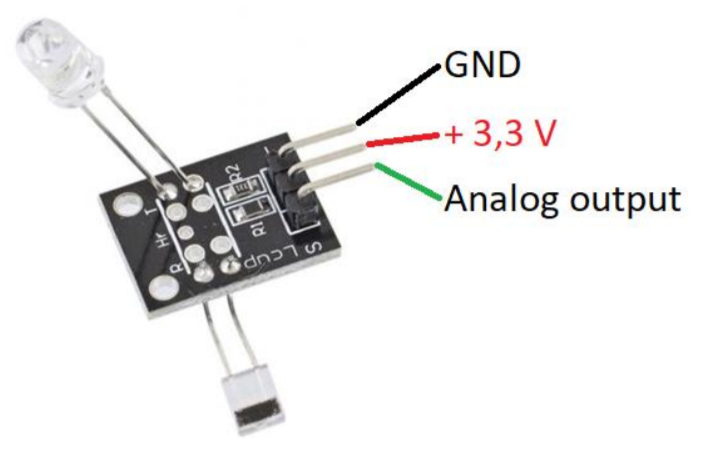
\includegraphics[width=220]{modulzapojeni.PNG}
    \caption{Popis modulu pro měření srdečního tepu, převzato z \cite{ZadaniPrezentace:web}}
  \end{minipage}
  \hspace{0.5cm}
  \begin{minipage}[b]{0.5\linewidth}
    \centering
    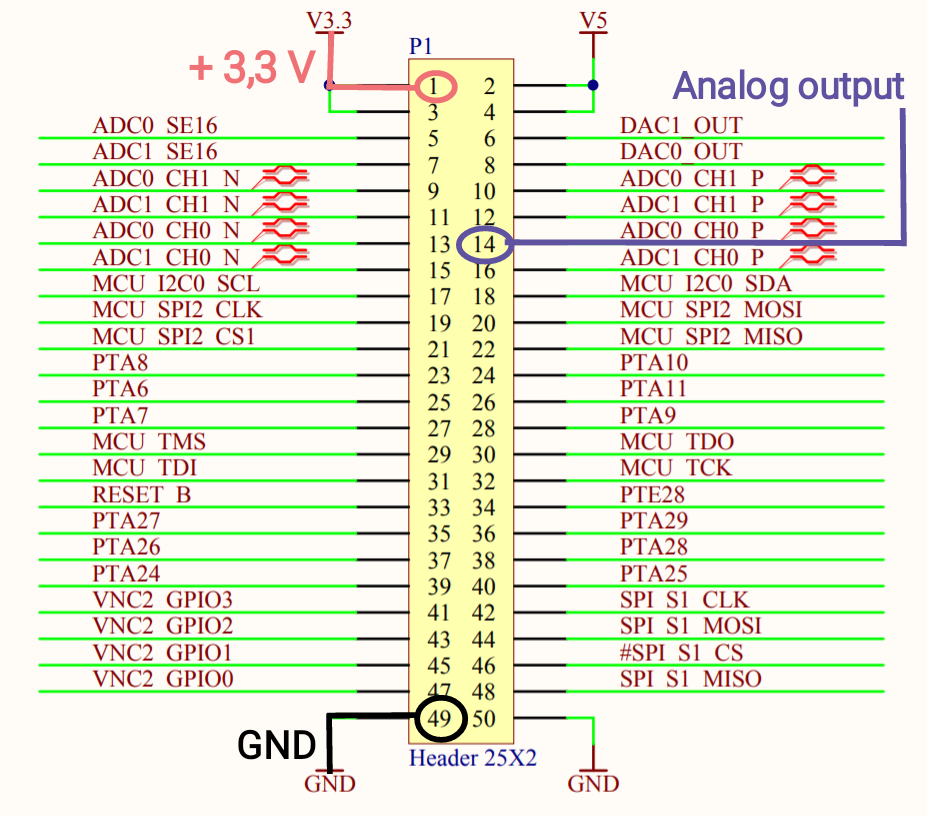
\includegraphics[width=200]{IMG_20191215_184411.png}
    \caption{Zapojení modulu, převzato a upraveno na základě manuálu pro FITKit3}
  \end{minipage}
\end{figure}


7-segmentový dispej byl pak zapojen na piny 17-28 pro P1. Displej byl pak rozdělen na jednotlivé číslice a následně jejich segmenty, kdy každá je připojena k určitému pinu. Každý segment jednotlivé číslice A - G je pak pojmenován jako \verb|DISPLAY_SEGMENT_písmeno|, například tedy \verb|DISPLAY_SEGMENT_A| pro segment A.  Rozdělení segmentů a číslic na maticovém displeji je pak následující:
\begin{figure}[htbp]
    \centering
    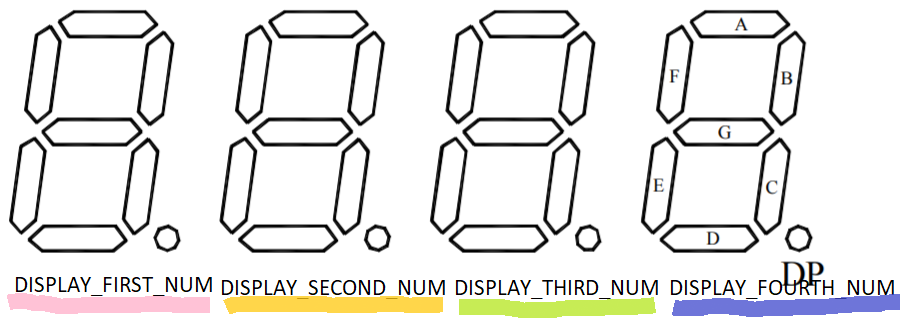
\includegraphics[width=260]{disp.png}
     \caption{7-segmentový displej použitý pro projekt, převzato z \cite{Displaydoc:web} a upraveno}
\end{figure}\\


Zapojení jednotlivých pinů pro displej byla vygenerována a následně upravena na základě MCUXpresso Config Tools, tento program umožňuje právě práci s potřebnou konfigurací pinů a jejich pojmenováním. Na~základě tohoto programu byl vygenerován obsah souboru \verb|pin_mux.c| a \verb|pin_mux.h| uložených ve složce \verb|boards|. Specifické piny pro zapojení každého segmentu a číslice na FITkitu v části P1 jsou následující, v závorce je pak uvedeno značení dle MCUXpresso Config Tools schématu):
\begin{itemize}
    \item pin 17 (C9) - zobrazení první číslice na displeji, pojmenováno jako \verb|DISPLAY_FIRST_NUM|
    \item pin 18 (B9) - zobrazení čtvrté číslice na displeji, pojmenováno jako \verb|DISPLAY_FOURTH_NUM|
    \item pin 19 (B1) - zobrazení třetí číslice na displeji, pojmenováno jako \verb|DISPLAY_THIRD_NUM|
    \item pin 20 (C3) - zobrazení druhé číslice na displeji, pojmenováno jako \verb|DISPLAY_SECOND_NUM|
    \item pin 21 (C1) - zobrazení segmentu G číslice, pojmenováno jako \verb|DISPLAY_SEGMENT_G|
    \item pin 22 (C2) - zobrazení segmentu C číslice, pojmenováno jako \verb|DISPLAY_SEGMENT_C|
    \item pin 23 (K8) - zobrazení desetinné tečky, nevyužito
    \item pin 24 (M9) - zobrazení segmentu D číslice, pojmenováno jako \verb|DISPLAY_SEGMENT_D|
    \item pin 25 (J7) - zobrazení segmentu E číslice, pojmenováno jako \verb|DISPLAY_SEGMENT_E|
    \item pin 26 (L9) - zobrazení segmentu A číslice, pojmenováno jako \verb|DISPLAY_SEGMENT_A|
    \item pin 27 (J8) - zobrazení segmentu F číslice, pojmenováno jako \verb|DISPLAY_SEGMENT_F|
    \item pin 28 (L8) - zobrazení segmentu B číslice, pojmenováno jako \verb|DISPLAY_SEGMENT_B|
\end{itemize}

\section{Popis způsobu řešení}
Program byl implementován v souboru \verb|main.c| ve složce \verb|sources|. Při implementaci jsem využila Kinetis Design Studio 3.0.0 IDE a SDK (Software Development Kit) vhodného právě pro práci s FITKitem3. 

Na začátku samotného běhu programu probíhá inicializace následujících komponent:
\begin{itemize}
    \item Inicializace nakonfigurovaných pinů GPIO (General-purpose input/output), jejichž implementace je v~souborech  \verb|pin_mux.c| a \verb|pin_mux.h|
    \item Inicializace PIT (Periodic Interrupt Timer) sloužící pro obnovování displeje po specifikované době
    \item Inicializace LPTMR (Low-Power Timer) pro práci s měřením časových intervalů a času při práci s~modulem srdečního tepu
    \item Inicializace ADC (16-bit successive Analog-to-Digital Converter) slouží pro převod analogového na~digitální signál získaného z modulu srdečního tepu
\end{itemize}

Řízení displeje probíhá na základě kontroly indexu čísla v řetězci, kdy zjistíme, s jakou ze čtyř číslic na~displeji se bude pracovat a následně se pak zjišťuje, které číslo je na této určité pozici (čísla 0 - 9). Na~základě tohoto určení se pak rozsvítí segmenty na displeji odpovídající právě určenému číslu (např. pro číslo 0 se rozsvítí všechny segmenty kromě segmentu G nebo pro číslo 1 se rozsvítí segment B a C, atd.). Typická frekvence pro obnovu displeje je 60 Hz. Čas pro obnovování displeje je vypočten následovně:\\
$$T = \frac{1}{f}$$
$$T = \frac{1}{60} = 0,016 s = 16666,667 \mu s$$
Displej obsahuje čtyři číslice, proto:\\
$$\frac{16666,667}{4} = 4166,667 \mu s$$

Obnovovací čas je tedy stanoven na 4167 mikrosekund. \\\\
Naměřený signál z modulu srdečního tepu je konvertován pomocí ADC a následně je filtrován dolní a poté horní propustí. Dolní propust slouží pro~odfiltrování signálu vyšších frekvencí, horní propust pak pro~odfiltování signálů nízkých frekvencí. Tyto filtry byly implementovány podle následujících pseudokódů:\\\\
Pseudokód pro dolní propust:\cite{Lowpass:web}
\begin{lstlisting}
 // Return RC low-pass filter output samples, given input samples,
 // time interval dt, and time constant RC
 function lowpass(real[0..n] x, real dt, real RC)
   var real[0..n] y
   var real alpha := dt / (RC + dt)
   y[0] := alpha * x[0]
   for i from 1 to n
       y[i] := alpha * x[i] + (1-alpha) * y[i-1]
   return y
\end{lstlisting}
Pseudokód pro horní propust:\cite{Highpass:web}
\begin{lstlisting}
 // Return RC high-pass filter output samples, given input samples,
 // time interval dt, and time constant RC
 function highpass(real[0..n] x, real dt, real RC)
   var real[0..n] y
   var real alpha := RC / (RC + dt)
   y[0] := x[0]
   for i from 1 to n
     y[i] := alpha * y[i-1] + alpha * (x[i] - x[i-1])
   return y
\end{lstlisting}

Signál je po přefiltrování měřen pouze v nejvyšším bodě, výsledek je pak ukládán do pole \verb|measured_values_arr|, po naměření třech po sobě jdoucích hodnot je spočítán jejich aritmetický průměr a je vypsán na displej. 
\section{Známé nedostatky}
I přes veškerou snahu nejsou naměřené hodnoty z modulu srdečního tepu úplně přesné, ačkoliv je více hodnot průměrováno před tím, než je vypsán finální výsledek a dokonce jsou zahozeny hodnoty nad 220 BPM a pod~60 BPM, což je maximální a minimální hodnota tepu pro člověka. Také měření ovlivňuje tlak na senzor, možný pohyb prstem nebo úhel přiložení.
\section{Závěr}
I přes ne úplnou přesnost zaznamenaného signálu se mi podařilo implementovat jak práci s 7-segmentovým displejem, tak filtrování pomocí horní a dolní propusti a následné spočítání a zobrazení výsledku na displej. 
\newpage
\bibliography{literatura}
\end{document}



\end{document}

